\documentclass{beamer}
% Use DS9 global theme
\usepackage{../../../../shared/templates/ds9_theme}

% Title page configuration
\title[ ]{PHYS11 CH:6.1-6.2}
\subtitle{ Circular \& Rotational Motion }
\author[Mr. Gullo]{Mr. Gullo}
\date[Oct 2024]{October 2024}

% Table of contents at the beginning of each section
\AtBeginSection[]
{
  \begin{frame}
    \frametitle{Table of Contents}
    \tableofcontents[currentsection]
  \end{frame}
}
\begin{document}

\frame{\titlepage}

\begin{frame}
\frametitle{Learning Objectives}
By the end of this lesson, you will be able to:
\begin{itemize}
    \item Define and calculate angle of rotation and angular velocity
    \item Understand uniform circular motion 
    \item Calculate centripetal acceleration and force
    \item Solve problems involving circular motion
\end{itemize}


\end{frame}

\section{Key Concepts}

\begin{frame}
\frametitle{Key Terms \& Definitions}
\begin{itemize}
    \item \textbf{Angle of Rotation} ($\Delta \theta$): Angular displacement measured in radians
       \item \textbf{Arc Length} ($\Delta s$): Distance traveled along circular path
    \item \textbf{Radius of Curvature} ($r$): Radius of circular path
   
\end{itemize}

\begin{figure}[H]
    \centering
    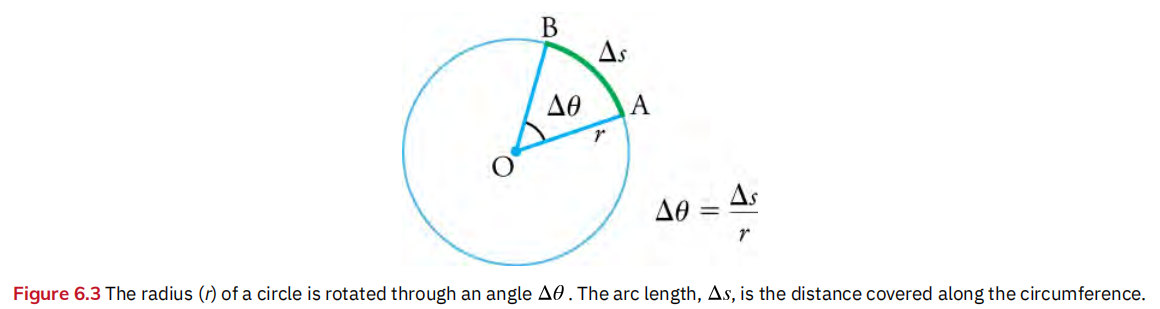
\includegraphics[width=1\linewidth]{Screenshot 2024-11-21 125544.png}
\end{figure}

\end{frame}


\begin{frame}
\frametitle{Key Terms \& Definitions}
\begin{itemize}
   
    \item \textbf{Angular Velocity} ($\omega$): Rate of change of angle with time
\begin{figure}[H]
    \centering
    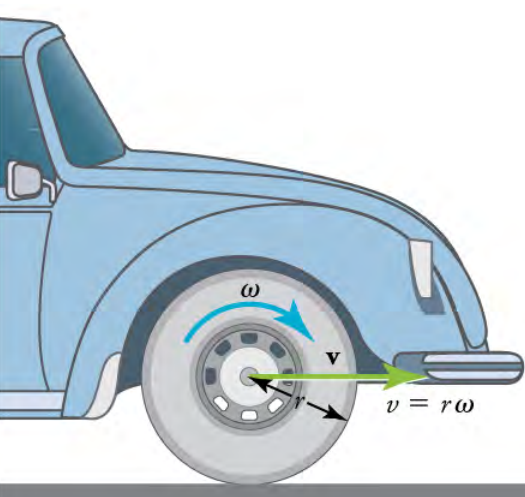
\includegraphics[width=0.6\linewidth]{Screenshot 2024-11-21 125846.png}
\end{figure}
\end{itemize}
\end{frame}

\begin{frame}
\begin{figure}
    \centering
    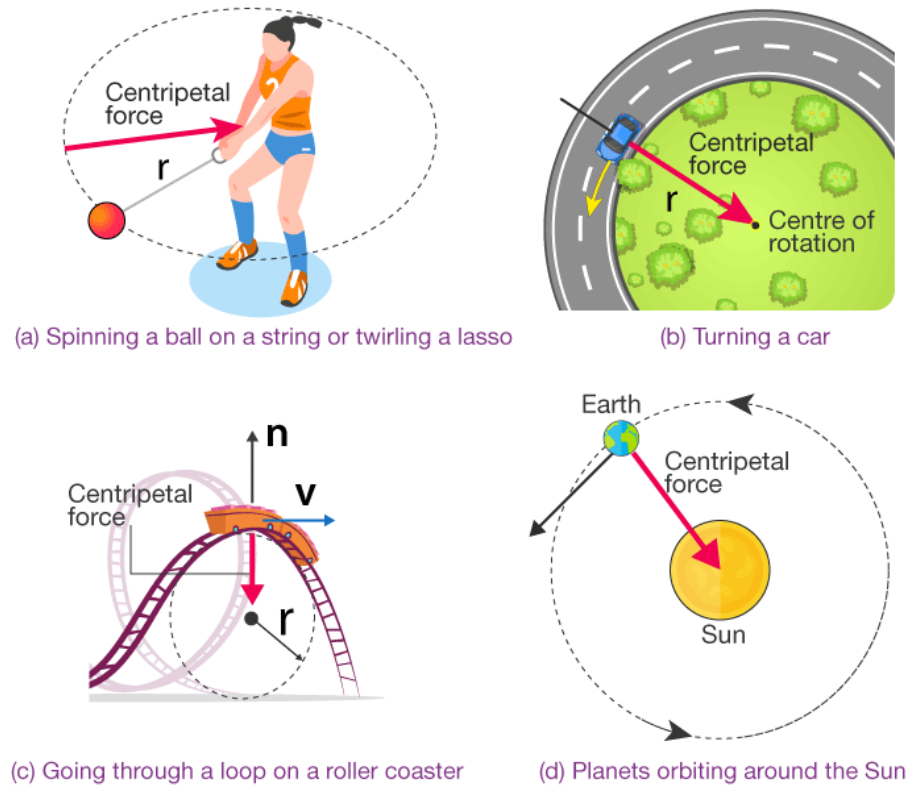
\includegraphics[width=0.8\linewidth]{Screenshot 2024-11-21 132156.png}
\end{figure}
\end{frame}

\begin{frame}
\frametitle{Key Terms \& Definitions}
\begin{itemize}
        \item \textbf{Centripetal Acceleration} ($a_c$): Acceleration toward center of circle
    \item \textbf{Centripetal Force} ($F_c$): Force causing circular motion
\begin{figure}
    \centering
    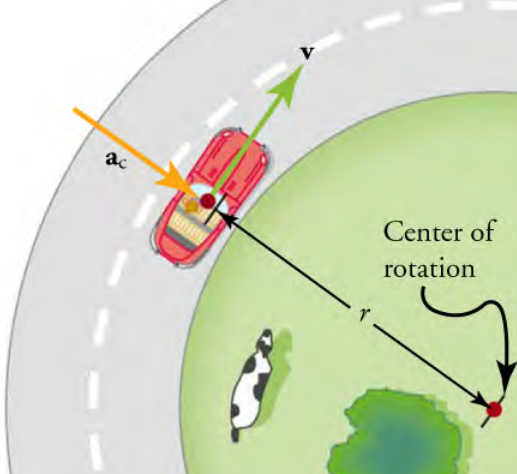
\includegraphics[width=0.7\linewidth]{Screenshot 2024-11-21 130344.png}
\end{figure}
    
\end{itemize}
\end{frame}

\begin{frame}

\frametitle{The Fictitious Centrifugal Force}

\begin{columns}[T]
\begin{column}{0.6\textwidth}
\textbf{What is the centrifugal "force"?}
\begin{itemize}
    \item Not a real force!
    \item Appears in rotating reference frames
    \item Feels like you're being "thrown outward"
\end{itemize}

\pause

\textbf{Examples in daily life:}
\begin{itemize}
    \item Car turning a corner
    \item Tea leaves gathering in center of cup
    \item Clothes in a washing machine
\end{itemize}
\end{column}

\begin{column}{0.4\textwidth}
% Simple TikZ diagram showing rotating reference frame
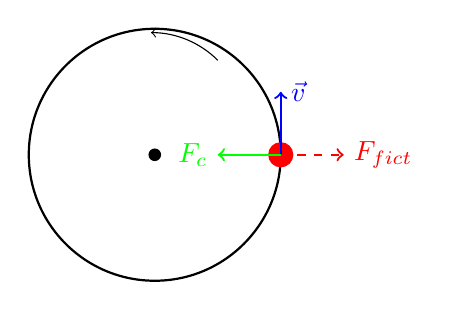
\begin{tikzpicture}[scale=0.8]
    % Draw circular path
    \draw[thick] (0,0) circle (2cm);
    
    % Draw rotating object
    \fill[red] (2,0) circle (0.2cm);
    
    % Draw velocity vector
    \draw[->,thick,blue] (2,0) -- (2,1) node[right] {$\vec{v}$};
    
    % Draw "fictitious force" vector
    \draw[->,thick,red,dashed] (2,0) -- (3,0) node[right] {$F_{fict}$};
    
    % Draw real centripetal force
    \draw[->,thick,green] (2,0) -- (1,0) node[left] {$F_c$};
    
    % Add center point
    \fill (0,0) circle (0.1cm);
    
    % Optional: Add curved arrow to show rotation
    \draw[->] (1,1.5) arc (45:90:1.5cm);
\end{tikzpicture}

\end{column}
\end{columns}

\vspace{0.3cm}
\end{frame}

\begin{frame}
    \textbf{Remember:}
\begin{itemize}
    \item Objects want to travel in straight lines (Newton's 1st Law)
    \item What we feel as "outward force" is actually inertia
    \item Real force is centripetal (inward), causing circular motion
\end{itemize}

\url{https://en.wikipedia.org/wiki/Centrifugal_force}

\end{frame}

\begin{frame}
\frametitle{Important Equations}
\begin{align*}
\text{Angle of Rotation:} & \quad \Delta \theta = \frac{\Delta s}{r} \\[1em]
\text{Angular Velocity:} & \quad \omega = \frac{\Delta \theta}{\Delta t} \\[1em]
\text{Tangential Velocity:} & \quad v = r\omega \\[1em]
\text{Centripetal Acceleration:} & \quad a_c = \frac{v^2}{r} = r\omega^2 \\[1em]
\text{Centripetal Force:} & \quad F_c = \frac{mv^2}{r} = mr\omega^2
\end{align*}
\end{frame}

\section{I Do}

\begin{frame}
\frametitle{I Do - Example}
A car drives around a circular track of radius 100 m at a constant speed of 20 m/s.
\begin{enumerate}
    \item Calculate the centripetal acceleration
    \item Find the centripetal force if the car's mass is 1500 kg
\end{enumerate}

\visible<2->{
Solution:
\begin{align*}
a_c &= \frac{v^2}{r} = \frac{(20\text{ m/s})^2}{100\text{ m}} = 4\text{ m/s}^2 \\[1em]
F_c &= ma_c = (1500\text{ kg})(4\text{ m/s}^2) = 6000\text{ N}
\end{align*}
}
\end{frame}

\section{We Do}

\begin{frame}
\frametitle{We Do - Together}
Let's solve this together: A CD spins at 300 rpm (revolutions per minute).
\begin{enumerate}
    \item Convert rpm to angular velocity in rad/s
    \item Calculate the tangential velocity at r = 6 cm
\end{enumerate}

\visible<2->{
Step 1: Convert rpm to rad/s
\[ \omega = 300\text{ rev/min} \times \frac{2\pi\text{ rad}}{1\text{ rev}} \times \frac{1\text{ min}}{60\text{ s}} = 31.4\text{ rad/s} \]
}

\visible<3->{
Step 2: Calculate tangential velocity
\[ v = r\omega = (0.06\text{ m})(31.4\text{ rad/s}) = 1.88\text{ m/s} \]
}
\end{frame}

\section{You Do}

\begin{frame}
\frametitle{You Do - Practice Problem}
A ball attached to a string is swung in a horizontal circle with radius 0.5 m. If the ball makes one complete revolution in 1.2 seconds:
\begin{enumerate}
    \item Calculate the angular velocity
    \item Find the centripetal acceleration
    \item Determine the tension in the string if the ball's mass is 0.2 kg
\end{enumerate}
\end{frame}

\begin{frame}
\frametitle{You Do - Solution}
\begin{enumerate}
    \item Angular velocity:
    \[ \omega = \frac{2\pi}{T} = \frac{2\pi\text{ rad}}{1.2\text{ s}} = 5.24\text{ rad/s} \]
    
    \item Centripetal acceleration:
    \[ a_c = r\omega^2 = (0.5\text{ m})(5.24\text{ rad/s})^2 = 13.7\text{ m/s}^2 \]
    
    \item Tension (centripetal force):
    \[ F_c = ma_c = (0.2\text{ kg})(13.7\text{ m/s}^2) = 2.74\text{ N} \]
\end{enumerate}
\end{frame}

\begin{frame}
\frametitle{Summary}
Key takeaways:
\begin{itemize}
    \item Circular motion requires centripetal force
    \item $a_c$ and $F_c$ always point toward center
    \item Angular quantities can be converted to linear quantities using radius
    \item Uniform circular motion means constant speed but changing velocity direction
\end{itemize}
\end{frame}

\end{document}
